\documentclass{beamer}
\usepackage{blindtext} 
\usetheme{Berkeley}
\usecolortheme{rose}
\usefonttheme{professionalfonts}
\setbeamercovered{dynamic}



\title{Beamer Assignment}
\subtitle{CS312 Assignemnt Week 2}
\author[T Satwik]{T Satwik \\ \texttt{190030043@iitdh.ac.in}}
\institute[CSE]{Computer Science \& Engineering, IIT Dharwad}           \date{08 September, 2020}
\logo{
\includegraphics[height=1cm]{logo.jpg}}

\begin{document}


\frame{\titlepage}



\section{Hyperlinks}  %<+->/pause overlay is used
\begin{frame}[label=Hyperlinks]{Hyperlinks}
\transdissolve    %transitions are used for every slide

\begin{itemize}[<+->] 
    \item The following link would direct you to the IIT Dharwad official website: \url{http://www.iitdh.ac.in}.
    \item The following link would direct you to the wikipedia page of IIT Dharwad: \url{https://en.wikipedia.org/wiki/Indian_Institute_of_Technology_Dharwad}.
    \item Click on the following button to view the slide where you can find the IIT Dharwad Pictures: \hyperlink{Figures}{\beamergotobutton{Go to Figures slide}}
    \item Click on the following button to view the table of 3rd semester CSE courses: \hyperlink{Table1}{\beamergotobutton{Go to courses table}}
    
\end{itemize}
\end{frame}



\section{Structure}  %onslide overlay is used here
\subsection{Columns}
\begin{frame}[label=Columns]{Structures : Columns}
\transblindshorizontal
    \begin{columns}
        \begin{column}{.45\textwidth}
            \onslide<1-> {\textbf{Heading 1} \\ Lorem ipsum dolor sit amet, consectetuer adipiscing elit. Aenean commodo ligula eget dolor. Aenean massa. Cum sociis natoque penatibus et magnis dis parturient montes, nascetur ridiculus mus. Donec quam felis, ultricies nec, pellentesque eu, pretium quis, sem. Nulla consequat massa quis enim. Donec pede justo, fringilla vel, aliquet nec, vulputate eget, arcu. }
        \end{column}
        
        \begin{column}{.45\textwidth}
            \onslide<2-> \textbf{Heading 2} \\Lorem ipsum dolor sit amet, consectetuer adipiscing elit. Aenean commodo ligula eget dolor. Aenean massa. Cum sociis natoque penatibus et magnis dis parturient montes, nascetur ridiculus mus. Donec quam felis, ultricies nec, pellentesque eu, pretium quis, sem. Nulla consequat massa quis enim. Donec pede justo, fringilla vel, aliquet nec, vulputate eget, arcu.
        \end{column}
    \end{columns}
\end{frame}



\subsection{Blocks} %only overlay is used
\begin{frame}[label=Blocks]{Structures : Blocks}
\transblindsvertical

    \only<1->{
    \begin{alertblock}{Heading 1}
        This is an example of  Alert block style.
    \end{alertblock}
    }
    \only<2->{
    \begin{block}{Heading 2}
        This is an example of default block style.
    \end{block}
    }
    
    \only<3->{
    \begin{exampleblock}{Heading 3}
        This is an example of  Example block style.
    \end{exampleblock}  
    }
    
\end{frame}



\section{Figures} %visible overlay is used
\begin{frame}[label=Figures]{Figures}
\transboxin
\begin{columns}
    
    \begin{column}{.45\textwidth}
    \visible<1->{
        \begin{block}{IITDh Logo}
			\begin{figure}
				\centering
				\includegraphics[width=1.5cm]{Logo.jpg}
			\end{figure}
		\end{block}
	}
    \end{column}
    
    
    \begin{column}{.45\textwidth}
    \visible<2->{
        \begin{block}{Campus Picture 1}
			\begin{figure}
				\centering
				
\includegraphics[height=1.5cm]{campus-1.jpg}
			\end{figure}
		\end{block}
	}
    \end{column}
    
\end{columns}
\visible<3->{
\begin{block}{Campus Picture 2}
    \begin{figure}
			\centering
			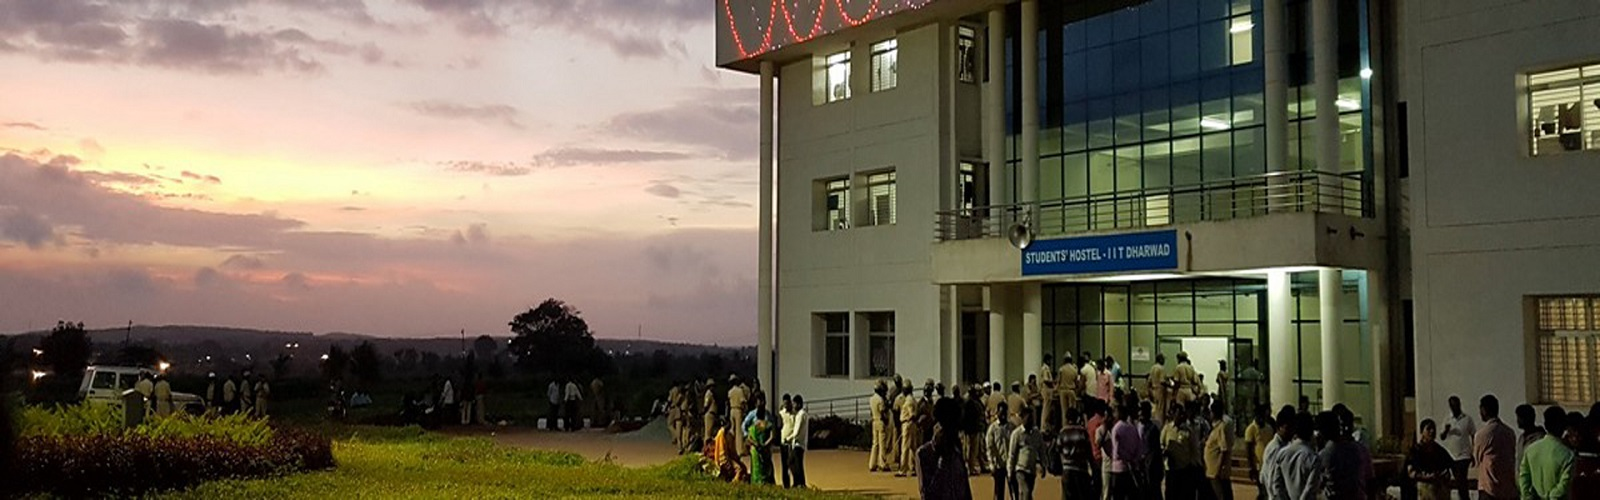
\includegraphics[height=1.8cm]{campus-2.jpg}
	\end{figure}
\end{block}
}
\end{frame}



\section{Tables} %pause overlay is used
\subsection{Table 1}
\begin{frame}[label=Table1]{Tables}
\transboxout

    \begin{table}[t]
        \centering
        \begin{tabular}{|c|c|c|c|}
            \hline
            Sl.No&Course Name&Code&Credits\\
            \hline
            \pause 1. & Data Structures and Algorithms & CS201 & 6 \\ \hline
            \pause 2. & Discrete Structures & CS203 & 6 \\
            \hline
            \pause 3. & Software Systems Lab & CS213 & 8 \\
            \hline
            \pause 4. & Data Structures and Algorithms Lab & CS211 & 3 \\
            \hline
            \pause 5. & Data Analysis & EE201 & 6 \\
            \hline
            \pause 6. & Economics & HS102 & 6\\
            \hline
        \end{tabular}
        \caption{3rd Sem Courses}
        \label{tab:3rdSemCourses}
    \end{table}
    
\end{frame}



\subsection{Table 2} %alert overlay is used
\begin{frame}[label=Table2]{Tables}
\transwipe
    
    \begin{table}                   %In this table the various types of lists are described
        \centering
        \begin{tabular}{| l| c |p{5cm} |}
            \hline
            sl. no & List Type & Description \\
            \hline
            1 & \alert<1>{itemize} & The lists are not ordered and each point is marked by a dot. \\
            1 & \alert<2>{enumerate} & The lists are ordered and each point is marked by a number automatically. \\
            1 & \alert<3>{description} & The lists are not ordered and each point is marked by a word you specify in "[ ]". \\
            \hline
         \end{tabular}
        \caption{Types of list}
        \label{tab:Types of lists}
    \end{table}
\end{frame}



\section{Math} %uncover overlay is used
\subsection{Theorems}
\begin{frame}[label=Theorems]{Math : Theorems and Proofs}
\transduration{2}
    
    \begin{theorem}
        \uncover<2->{For  a given angle $ \theta, \sin^2\theta  + \cos^2\theta = 1$}
    \end{theorem}
    
    \begin{theorem}
        \uncover<2->{Sum of first $n$ natural numbers is given by $\frac{n(n+1)}{2}$} 
    \end{theorem}
\end{frame}



\subsection{Proof} %pause and onslide are used
\begin{frame}[label=Proof]{Math : Theorems and Proofs}
\transblindshorizontal
    \pause
    \begin{proof}
        \onslide<2->
        Lets us assume that the sum of first n natural numbers$ = T(n)$
        \begin{equation}
            T(n)= 1 + 2 + .... n
        \end{equation}
        
        \onslide<3->
        $T(n)$ can also be written as follows
        \begin{equation}
            T(n) = n + n-1 + .... 1
        \end{equation}
        
        \onslide<4->
        Adding the above equations we get
        \begin{eqnarray*}
            2*T(n) = (n+1) + (n+1) + .... (n+1) \\
            \implies T(n) = \frac{n(n+1)}{2}
        \end{eqnarray*}
    \end{proof}
\end{frame}



\subsection{Multiline Equation with Step wise Viewing} %onslide overlay is used
\begin{frame}[label=Multiline Equations]{Math : Multiline Equation with Step wise Viewing}
\transblindshorizontal
    Factorization of Quadratic Equations:
    \begin{eqnarray*}
        \onslide<2->x^2 + 2x - 3 = 0 \\
        \onslide<3->x^2 + 3x - x - 3 = 0 \\
        \onslide<4->x(x+3) -1(x+3) = 0 \\
        \onslide<5->(x-1)(x+3) = 0 
    \end{eqnarray*}
    
\end{frame}



\section{Lists}   %Alert and Color overlays are used.
\begin{frame}[label= Lists]{Lists}
\transblindshorizontal
    \alert<1>{This is an Example of itemize}
    \begin{itemize}
        \color<1>{green}{
        \item The first point with Itemize style of formatting.
        \item The second point with Itemize style of formatting.
        }
    \end{itemize}
    \alert<2>{This is an Example of enumerate}
    \begin{enumerate}
        \color<2>{blue}{
        \item The first point with enumerate style of formatting.
        \item The second point with enumerate style of formatting. 
        }
    \end{enumerate}
    
    \alert<3>{This is an Example of description}
    \begin{description}
        \color<3>{orange}{
        \item [First] The first point with Description style of formatting.
        \item [Second] The second point with Description style of formatting.
        }
    \end{description}
\end{frame}

\end{document}